\cleardoublepage



\chapter{Introduction de l'étude}

%%%%%%%%%%%%%%%%%%%%%%%%%%%%%%%%%%%%%%%%%%%%%%%%%%%%%%%%%%%%%%%%%%%%%%%%%%%%%%%%%%%%%%%%%%%%%%%%%%%%
%%%%%%%%%%%%%%%%%%%%%%%%%%%%%%%%%%%%%%%%%%%%%%%%%%%%%%%%%%%%%%%%%%%%%%%%%%%%%%%%%%%%%%%%%%%%%%%%%%%%
%%%%%%%%%%%%%%%%%%%%%%%%%%%%%%%%%%%%%%%%%%%%%%%%%%%%%%%%%%%%%%%%%%%%%%%%%%%%%%%%%%%%%%%%%%%%%%%%%%%%
%%%%%%%%%%%%%%%%%%%%%%%%%%%%%%%%%%%%%%%%%%%%%%%%%%%%%%%%%%%%%%%%%%%%%%%%%%%%%%%%%%%%%%%%%%%%%%%%%%%%
%%%%%%%%%%%%%%%%%%%%%%%%%%%%%%%%%%%%%%%%%%%%%%%%%%%%%%%%%%%%%%%%%%%%%%%%%%%%%%%%%%%%%%%%%%%%%%%%%%%%

\section{Présentation de l'entreprise}

%%%%%%%%%%%%%%%%%%%%%%%%%%%%%%%%%%%%%%%%%%%%%%%%%%%%%%%%%%%%%%%%%%%%%%%%%%%%%%%%%%%%%%%%%%%%%%%%%%%%
%%%%%%%%%%%%%%%%%%%%%%%%%%%%%%%%%%%%%%%%%%%%%%%%%%%%%%%%%%%%%%%%%%%%%%%%%%%%%%%%%%%%%%%%%%%%%%%%%%%%
%%%%%%%%%%%%%%%%%%%%%%%%%%%%%%%%%%%%%%%%%%%%%%%%%%%%%%%%%%%%%%%%%%%%%%%%%%%%%%%%%%%%%%%%%%%%%%%%%%%%

\subsection{L'entreprise}

Le groupe \href{http://www.hutchinson.fr}{Hutchinson} est une entreprise spécialisée dans la transformation du caoutchouc industriel, dont l'innovation est l'objectif principal.
Plusieurs domaines de compétences et technologiques sont mis en œuvre par l'entreprise :
\begin{itemize}
	\item l'étanchéité,
	\item l'isolation (thermique, acoustique, ou vibratoire),
	\item le transfert de fluides,
	\item la transmission et la mobilité,
	\item la protection et les soins.
\\
\end{itemize}


Hutchinson est implanté dans 20 pays dans le monde, avec plus de 29.000 collaborateurs répartis dans 91 sites.

En 2011, son chiffre d'affaires s'élève à 2.987 millions d'euros, dont 64\% provient du secteur de la transmission et mobilité, et 63\% en Europe.
\\


Créée en 1853, l'entreprise devient une filiale de Total, 5\up{ème} groupe pétrolier mondial, suite à la prise majoritaire des parts du groupe Hutchinson.
\\




%%%%%%%%%%%%%%%%%%%%%%%%%%%%%%%%%%%%%%%%%%%%%%%%%%%%%%%%%%%%%%%%%%%%%%%%%%%%%%%%%%%%%%%%%%%%%%%%%%%%
%%%%%%%%%%%%%%%%%%%%%%%%%%%%%%%%%%%%%%%%%%%%%%%%%%%%%%%%%%%%%%%%%%%%%%%%%%%%%%%%%%%%%%%%%%%%%%%%%%%%
%%%%%%%%%%%%%%%%%%%%%%%%%%%%%%%%%%%%%%%%%%%%%%%%%%%%%%%%%%%%%%%%%%%%%%%%%%%%%%%%%%%%%%%%%%%%%%%%%%%%

\subsection{Recherche et développement (R\&D)}

La R\&D (Recherche et Développement) est un point fort du groupe Hutchinson.
En effet, cela permet à l'entreprise de concevoir des produits à la pointe de la technologie, et de rester le plus compétitif.
30 brevets ont ainsi été déposés en 2010.
\\


Le groupe Hutchinson possède un centre de recherche, basé à Montargis à proximité de Paris (France), ainsi que 26 centres de développement techniques dans le monde.
\\


Au total, ce sont près de 2.000 ingénieurs et techniciens qui travaillent dans la R\&D, majoritairement dans le domaine de la chimie, la physique et la mécanique.
L'entreprise y consacre 144 millions d'euros en 2011, soit 4,8\% de son chiffre d'affaire, mais aussi 15\% de ses ressources.
\\




%%%%%%%%%%%%%%%%%%%%%%%%%%%%%%%%%%%%%%%%%%%%%%%%%%%%%%%%%%%%%%%%%%%%%%%%%%%%%%%%%%%%%%%%%%%%%%%%%%%%
%%%%%%%%%%%%%%%%%%%%%%%%%%%%%%%%%%%%%%%%%%%%%%%%%%%%%%%%%%%%%%%%%%%%%%%%%%%%%%%%%%%%%%%%%%%%%%%%%%%%
%%%%%%%%%%%%%%%%%%%%%%%%%%%%%%%%%%%%%%%%%%%%%%%%%%%%%%%%%%%%%%%%%%%%%%%%%%%%%%%%%%%%%%%%%%%%%%%%%%%%

\subsection{Lieu du stage}

Le développement de logiciel de simulation est un des secteurs d'activité de la R\&D.
\\


Le stage s'est effectué dans le centre de simulation numérique, situé à Levallois-Perret (France).
Le service est composé de 2 ingénieurs, et emploie plusieurs intervenants extérieurs, qui sont chargés de développer et maintenir les nombreux logiciels utilisés par les différents secteurs de l'entreprise :
\begin{itemize}
	\item les logiciels métier, utilisés par les industriels,
	\item les logiciels de simulation numérique, utilisés principalement dans le centre de recherche.
\\
\end{itemize}





%%%%%%%%%%%%%%%%%%%%%%%%%%%%%%%%%%%%%%%%%%%%%%%%%%%%%%%%%%%%%%%%%%%%%%%%%%%%%%%%%%%%%%%%%%%%%%%%%%%%
%%%%%%%%%%%%%%%%%%%%%%%%%%%%%%%%%%%%%%%%%%%%%%%%%%%%%%%%%%%%%%%%%%%%%%%%%%%%%%%%%%%%%%%%%%%%%%%%%%%%
%%%%%%%%%%%%%%%%%%%%%%%%%%%%%%%%%%%%%%%%%%%%%%%%%%%%%%%%%%%%%%%%%%%%%%%%%%%%%%%%%%%%%%%%%%%%%%%%%%%%
%%%%%%%%%%%%%%%%%%%%%%%%%%%%%%%%%%%%%%%%%%%%%%%%%%%%%%%%%%%%%%%%%%%%%%%%%%%%%%%%%%%%%%%%%%%%%%%%%%%%
%%%%%%%%%%%%%%%%%%%%%%%%%%%%%%%%%%%%%%%%%%%%%%%%%%%%%%%%%%%%%%%%%%%%%%%%%%%%%%%%%%%%%%%%%%%%%%%%%%%%
%%%%%%%%%%%%%%%%%%%%%%%%%%%%%%%%%%%%%%%%%%%%%%%%%%%%%%%%%%%%%%%%%%%%%%%%%%%%%%%%%%%%%%%%%%%%%%%%%%%%

\section{Qu'est ce que la virtualisation ?}

Avant de commencer ce rapport, quelques explications sur la virtualisation permettront de mieux comprendre cette solution, sur laquelle se base mon projet.
\\




%%%%%%%%%%%%%%%%%%%%%%%%%%%%%%%%%%%%%%%%%%%%%%%%%%%%%%%%%%%%%%%%%%%%%%%%%%%%%%%%%%%%%%%%%%%%%%%%%%%%
%%%%%%%%%%%%%%%%%%%%%%%%%%%%%%%%%%%%%%%%%%%%%%%%%%%%%%%%%%%%%%%%%%%%%%%%%%%%%%%%%%%%%%%%%%%%%%%%%%%%
%%%%%%%%%%%%%%%%%%%%%%%%%%%%%%%%%%%%%%%%%%%%%%%%%%%%%%%%%%%%%%%%%%%%%%%%%%%%%%%%%%%%%%%%%%%%%%%%%%%%

\subsection{Objectif}

La virtualisation consiste à émuler un ou plusieurs systèmes d'exploitation sur un même ordinateur.

Il est ainsi possible d'utiliser par exemple Linux au sein même d'un environnement Windows.
\\


On appelle "machine hôte" (ou "l'hôte") le système principal installé sur l'ordinateur, et on appelle "machine virtuelle" le système d'exploitation qui sera virtualisé et qui fonctionnement au sein de la machine hôte.

Dans ce projet, Windows sera la machine hôte et Linux sera la machine virtuelle.
\\


\begin{figure}[!h]
	\center
	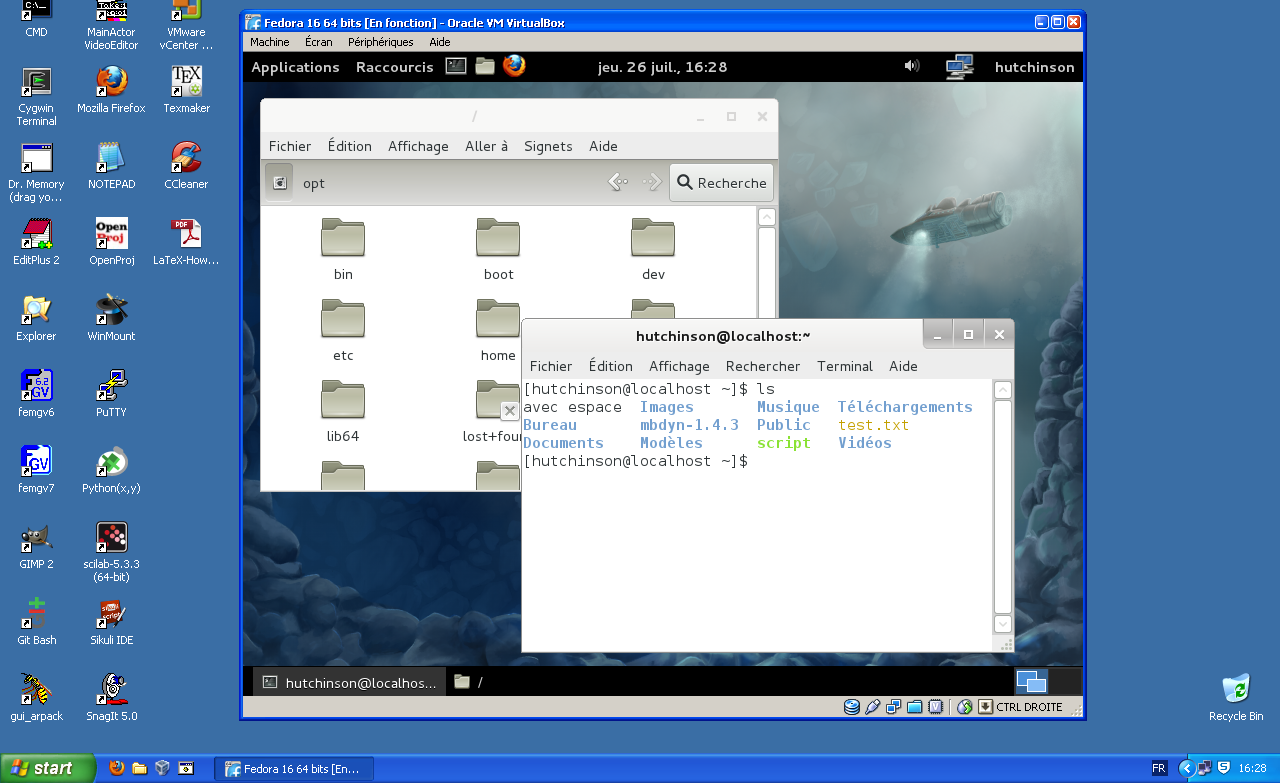
\includegraphics[scale=0.35]{images/Virtualisation.png}
	\caption{Système d'exploitation Linux virtualisé dans un environnement hôte Windows}
	\label{Screenshot Virtualisation}
\end{figure}

La capture d'écran \ref{Screenshot Virtualisation} illustre simplement le principe de la virtualisation.
Il s'agit du système d'exploitation Linux (Fedora 16) fonctionnant à l'intérieur d'une simple fenêtre Windows.
\\




%%%%%%%%%%%%%%%%%%%%%%%%%%%%%%%%%%%%%%%%%%%%%%%%%%%%%%%%%%%%%%%%%%%%%%%%%%%%%%%%%%%%%%%%%%%%%%%%%%%%
%%%%%%%%%%%%%%%%%%%%%%%%%%%%%%%%%%%%%%%%%%%%%%%%%%%%%%%%%%%%%%%%%%%%%%%%%%%%%%%%%%%%%%%%%%%%%%%%%%%%
%%%%%%%%%%%%%%%%%%%%%%%%%%%%%%%%%%%%%%%%%%%%%%%%%%%%%%%%%%%%%%%%%%%%%%%%%%%%%%%%%%%%%%%%%%%%%%%%%%%%

\subsection{Fonctionnement}

Le principe général de la virtualisation consiste à créer une interface, ou couche d'abstraction, entre le matériel de l'ordinateur et le système virtualisé.
Cette couche est appelée \textit{hyperviseur}.

Il existe plusieurs techniques différentes permettant la virtualisation.
Ce qui les différencie est le degré d'abstraction et l'agencement des couches.
Les deux types de virtualisations les plus utilisés vous sont présentés ici. 
\\



%%%%%%%%%%%%%%%%%%%%%%%%%%%%%%%%%%%%%%%%%%%%%%%%%%%%%%%%%%%%%%%%%%%%%%%%%%%%%%%%%%%%%%%%%%%%%%%%%%%%

\subsubsection{Hyperviseur de type 1}

\begin{figure}[!h]
	\center
	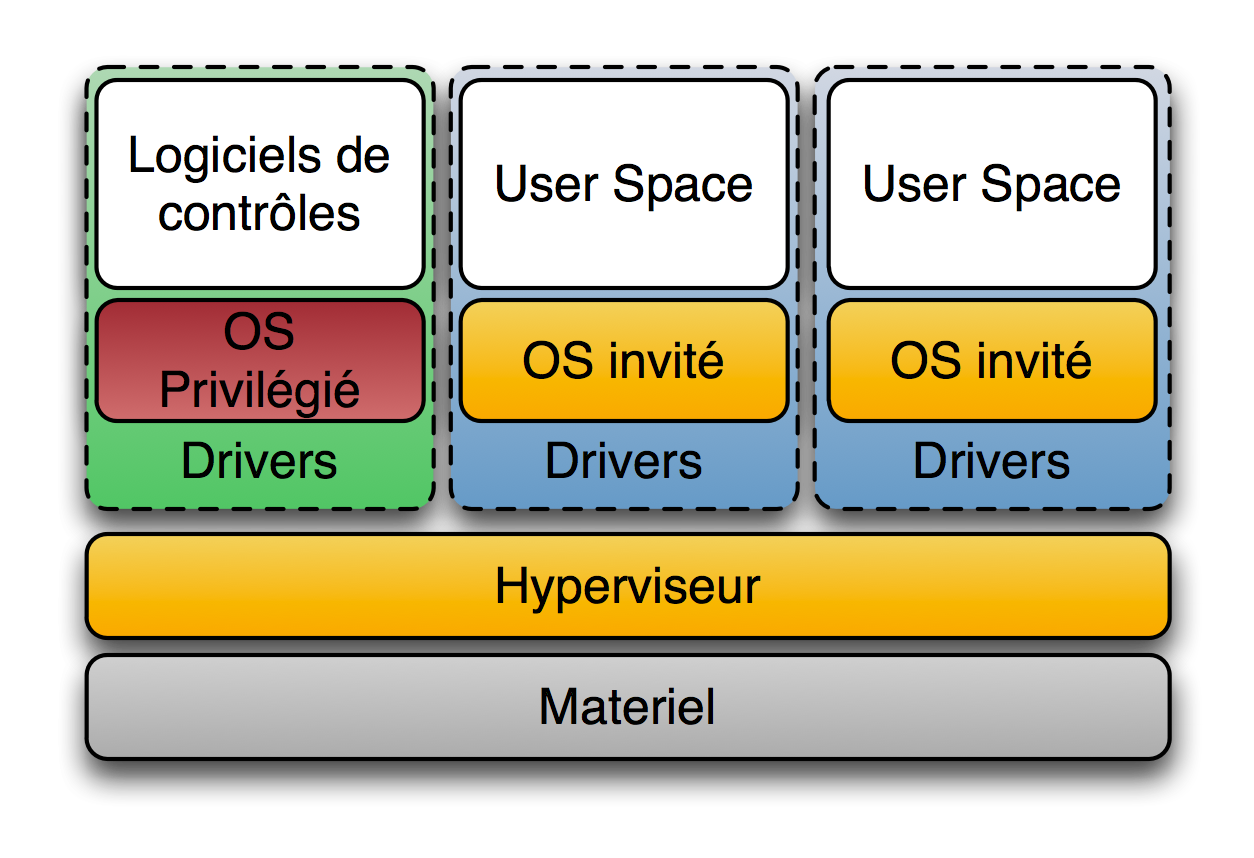
\includegraphics[scale=0.7]{images/Hyperviseur_type1.png}
	\caption{Hyperviseur de type 1}
	Source : Wikipédia - \href{http://fr.wikipedia.org/wiki/Virtualisation}{http://fr.wikipedia.org/wiki/Virtualisation}
	\label{Schéma Hyperviseur 1}
\end{figure}

Le premier type de virtualisation est appelé \textit{hyperviseur de type 1}.
L'hyperviseur permet de gérer l'accès des noyaux invités au matériel, comme présenté dans la figure \ref{Schéma Hyperviseur 1}.

Cette technique est la plus performante bien que coûteuse et compliquée à mettre en place.
Elle est principalement utilisée sur des serveurs qui disposent de plusieurs fonctions regroupées sur une même machine par gain d'énergie ou d'investissement.
\\



%%%%%%%%%%%%%%%%%%%%%%%%%%%%%%%%%%%%%%%%%%%%%%%%%%%%%%%%%%%%%%%%%%%%%%%%%%%%%%%%%%%%%%%%%%%%%%%%%%%%

\subsubsection{Hyperviseur de type 2}

\begin{figure}[!h]
	\center
	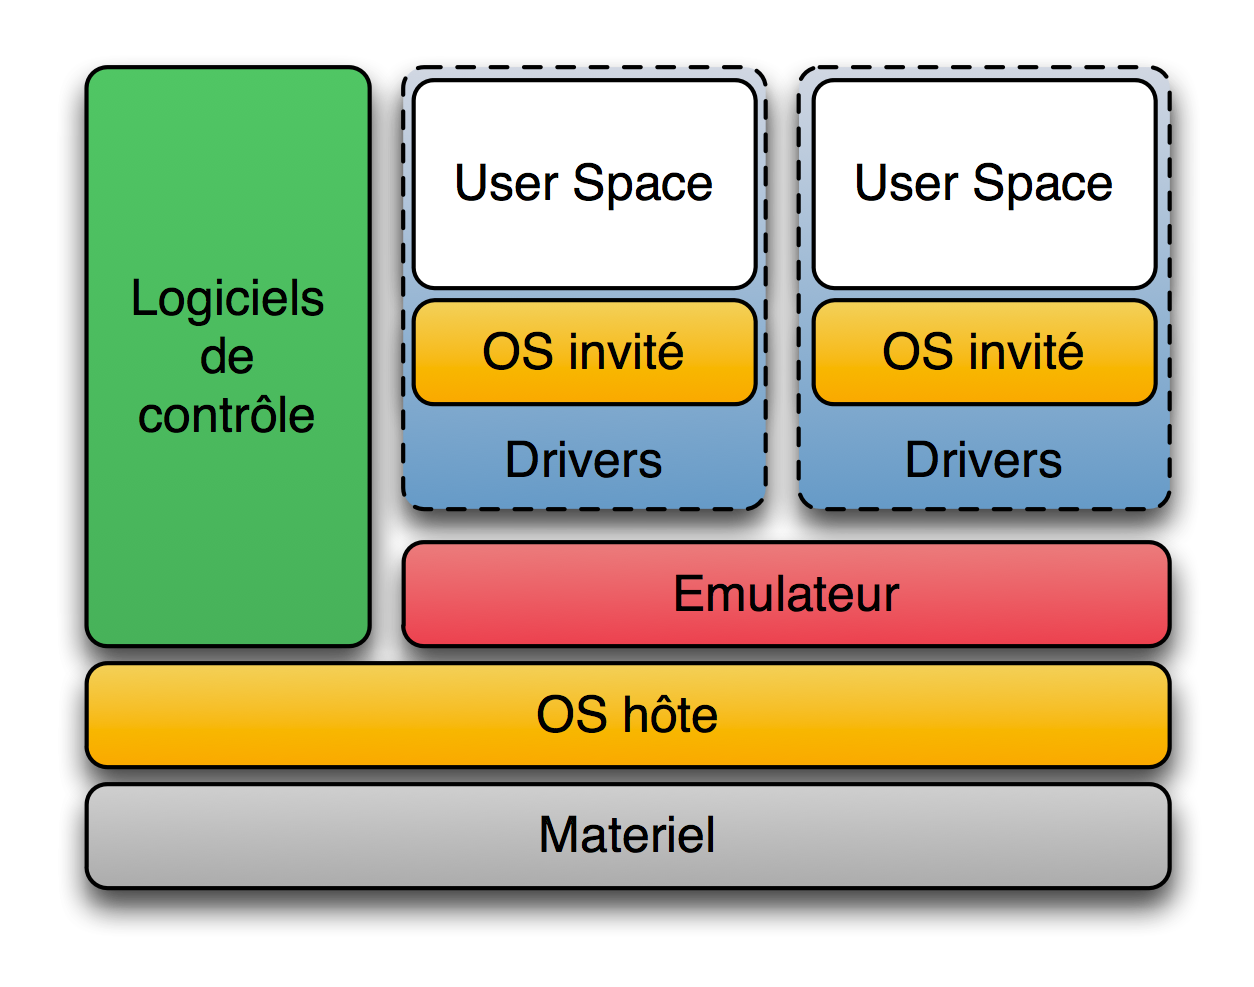
\includegraphics[scale=0.7]{images/Hyperviseur_type2.png}
	\caption{Hyperviseur de type 2}
	Source : Wikipédia - \href{http://fr.wikipedia.org/wiki/Virtualisation}{http://fr.wikipedia.org/wiki/Virtualisation}
	\label{Schéma Hyperviseur 2}
\end{figure}

Dans cette technique, l'hyperviseur est un logiciel fonctionnant sur le système d'exploitation hôte (voir figure \ref{Schéma Hyperviseur 2}).
Il a pour but de virtualiser ou d'émuler les composants de l'ordinateur (processeur, mémoire vive, mais aussi carte graphique, carte son, carte réseau, \ldots).
Ainsi, les machines virtuelles fonctionneront comme si elles communiquaient avec de vrais composants.

Bien que les performances des machines virtuelles soient inférieures au type 1, cette solution est très simple à mettre en place car elle nécessite principalement l'installation du logiciel de virtualisation.
\\


Dans ce projet, il s'agira d'utiliser cette technique de virtualisation pour réaliser la solution.
Nous nous restreindrons donc à l'hyperviseur de type 2 dans la suite de ce rapport.
\\




%%%%%%%%%%%%%%%%%%%%%%%%%%%%%%%%%%%%%%%%%%%%%%%%%%%%%%%%%%%%%%%%%%%%%%%%%%%%%%%%%%%%%%%%%%%%%%%%%%%%
%%%%%%%%%%%%%%%%%%%%%%%%%%%%%%%%%%%%%%%%%%%%%%%%%%%%%%%%%%%%%%%%%%%%%%%%%%%%%%%%%%%%%%%%%%%%%%%%%%%%
%%%%%%%%%%%%%%%%%%%%%%%%%%%%%%%%%%%%%%%%%%%%%%%%%%%%%%%%%%%%%%%%%%%%%%%%%%%%%%%%%%%%%%%%%%%%%%%%%%%%

\subsection{Particularités de la virtualisation}
\label{Particularités de la virtualisation}

Plusieurs particularités seront mis en évidence et développées tout au long de ce rapport.
\\



%%%%%%%%%%%%%%%%%%%%%%%%%%%%%%%%%%%%%%%%%%%%%%%%%%%%%%%%%%%%%%%%%%%%%%%%%%%%%%%%%%%%%%%%%%%%%%%%%%%%

\subsubsection{Les composants virtualisés}
\label{Les composants virtualisés}

Dans le cas d'une machine physique, la modification des performances demande un changement des composants, tels que le processeur, les barrettes de RAM, la carte graphique, \ldots.

L'avantage de la virtualisation, dans le cas de l'hyperviseur de type 2, repose sur le fait que les composants matériels sont virtualisés ou émulés par l'hyperviseur.
Ainsi, il est possible de régler facilement les performances de la machine virtuelle en modifiant les ressources allouées.
Cela se fait généralement en utilisant les outils de configuration mis à disposition par le logiciel de virtualisation.
\\


Selon le logiciel utilisé, les composants seront virtualisés ou émulés.
La virtualisation possède toutefois des performances plus élevées que l'émulation.
\\



%%%%%%%%%%%%%%%%%%%%%%%%%%%%%%%%%%%%%%%%%%%%%%%%%%%%%%%%%%%%%%%%%%%%%%%%%%%%%%%%%%%%%%%%%%%%%%%%%%%%

\subsubsection{Les disques virtuels}
\label{Les disques virtuels}

On appelle \textit{disque virtuel} la mémoire allouée permettant d'émuler un disque dur.

\begin{figure}[!h]
	\center
	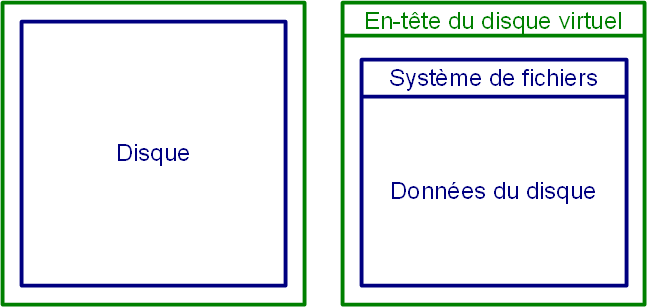
\includegraphics[scale=0.5]{images/Disque_virtuel.png}
	\caption{Schéma de la structure d'un disque virtuel}
	\label{Schéma Disque virtuel}
\end{figure}

Le disque virtuel sera modélisé sous forme d'un fichier (d'extension \textit{.vdi}) présent dans l'arborescence du système d'exploitation hôte.
Ce fichier encapsule un disque, et est composé de plusieurs parties :
\begin{itemize}
	\item un en-tête, contenant plusieurs informations sur la structure du fichier ;
	\item la structure d'un disque composé du système de fichiers et des données associées.
\end{itemize}
La figure \ref{Schéma Disque virtuel} schématise la structure globale du fichier.
\\


Comme pour les machines physiques où l'on peut brancher des disques durs sur des ports SATA\footnote{SATA (Serial Advanced Technology Attachment) : Norme utilisée pour l'échange de données entre les cartes mères et les stockages de masse. Donne son nom aux ports utilisés pour le branchement des disques car un "câble SATA" est nécessaire.} de la carte mère, il est possible d'ajouter des disques virtuels à la machine virtuelle pour émuler l'ajout d'un disque dur.
Cette action est effectuée par l'hyperviseur, et la machine virtuelle le considérera comme un vrai disque.
\\



%%%%%%%%%%%%%%%%%%%%%%%%%%%%%%%%%%%%%%%%%%%%%%%%%%%%%%%%%%%%%%%%%%%%%%%%%%%%%%%%%%%%%%%%%%%%%%%%%%%%

\subsubsection{Les types de réseau}
\label{Les types de réseau}

La carte réseau est un des composant nécessaire à la machine virtuelle pour accéder à la machine hôte ou au réseau extérieur.
Le composant est virtualisé (voir partie \ref{Les composants virtualisés}), ce qui permet de définir quel type de réseau sera établi entre la machine hôte et la machine virtuelle.
\\


\paragraph{Accès privé hôte :}

Chacune des machines virtuelles a accès à la machine hôte, mais n'a aucun accès à l'extérieur du réseau (schéma \ref{Schéma Accès privé hôte}).
Ce type de réseau ne permet pas d'accéder à internet, et les machines virtuelles ne sont pas joignables depuis l'extérieur.

\begin{figure}[H]
	\center
	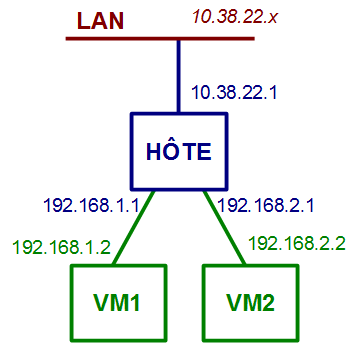
\includegraphics[scale=0.5]{images/types_reseau/Acces_prive_hote.png}
	\caption{Réseau de type "Accès privé hôte"}
	\label{Schéma Accès privé hôte}
\end{figure}


\paragraph{Réseau interne :}

Ce mode permet de créer un nouveau réseau privé entre les différentes machines virtuelles de la machine hôte (schéma \ref{Schéma Réseau interne}).
Les machines virtuelles n'auront accès qu'à ce réseau, et ne pourront pas accéder au LAN ni à internet.

\begin{figure}[H]
	\center
	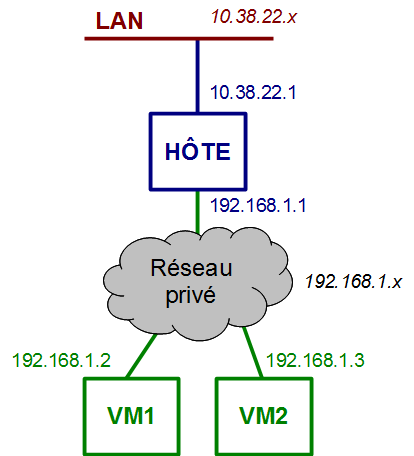
\includegraphics[scale=0.5]{images/types_reseau/Reseau_interne.png}
	\caption{Réseau de type "Réseau interne"}
	\label{Schéma Réseau interne}
\end{figure}


\paragraph{NAT :}

Les trames de la machine virtuelle transiteront par le biais de la machine hôte, qui servira de routeur.
Une translation d'adresse (NAT, Network Address Translation) sera effectuée, et les paquets possèderont la même adresse IP que la machine hôte. (schéma \ref{Schéma NAT})

La machine virtuelle aura accès au réseau LAN, mais vu du LAN la machine virtuelle n'existera pas.
Elle ne pourra pas être utilisée comme serveur, mais uniquement comme client.

Ce type de réseau est le plus pratique pour accéder à internet et pour une utilisation basique, sur un réseau sans configuration spéciale (proxy, IP fixe, \ldots).

\begin{figure}[H]
	\center
	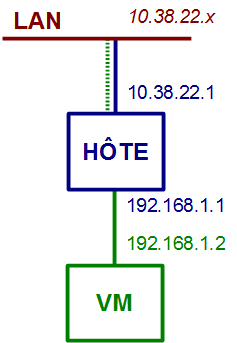
\includegraphics[scale=0.5]{images/types_reseau/NAT.png}
	\caption{Réseau de type "NAT"}
	\label{Schéma NAT}
\end{figure}


\paragraph{Accès par pont (bridge) :}

Ce mode est le plus complet, car il permet à la machine virtuelle d'apparaitre sur le réseau comme s'il s'agissait d'une nouvelle machine (schéma \ref{Schéma Accès par pont}).
Elle possèdera ainsi sa propre adresse IP et adresse MAC, et sera accessible par les machines du LAN.
Il est ainsi possible d'utiliser la machine virtuelle comme serveur.

\begin{figure}[H]
	\center
	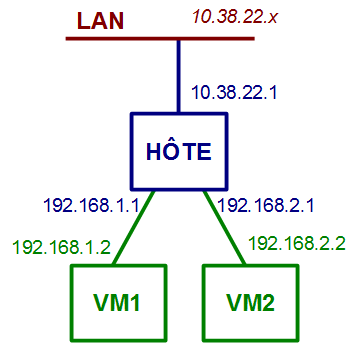
\includegraphics[scale=0.5]{images/types_reseau/Acces_prive_hote.png}
	\caption{Réseau de type "Accès par pont"}
	\label{Schéma Accès par pont}
\end{figure}
~~\\



%%%%%%%%%%%%%%%%%%%%%%%%%%%%%%%%%%%%%%%%%%%%%%%%%%%%%%%%%%%%%%%%%%%%%%%%%%%%%%%%%%%%%%%%%%%%%%%%%%%%

\subsubsection{Le répertoire partagé}
\label{Le répertoire partagé}

Il est possible de partager un répertoire, appelé \textit{répertoire partagé}, entre la machine hôte et la machine virtuelle.
Le contenu sera ainsi disponible "simultanément" sur la machine hôte et la machine virtuelle.

Le principe est le même que le "répertoire partagé" du réseau Windows, où les utilisateurs du réseau pourront accéder au répertoire, à l'exception qu'il ne demande aucune configuration particulière (droits d'accès, réseau, \ldots).
\\


\begin{figure}[!h]
	\center
	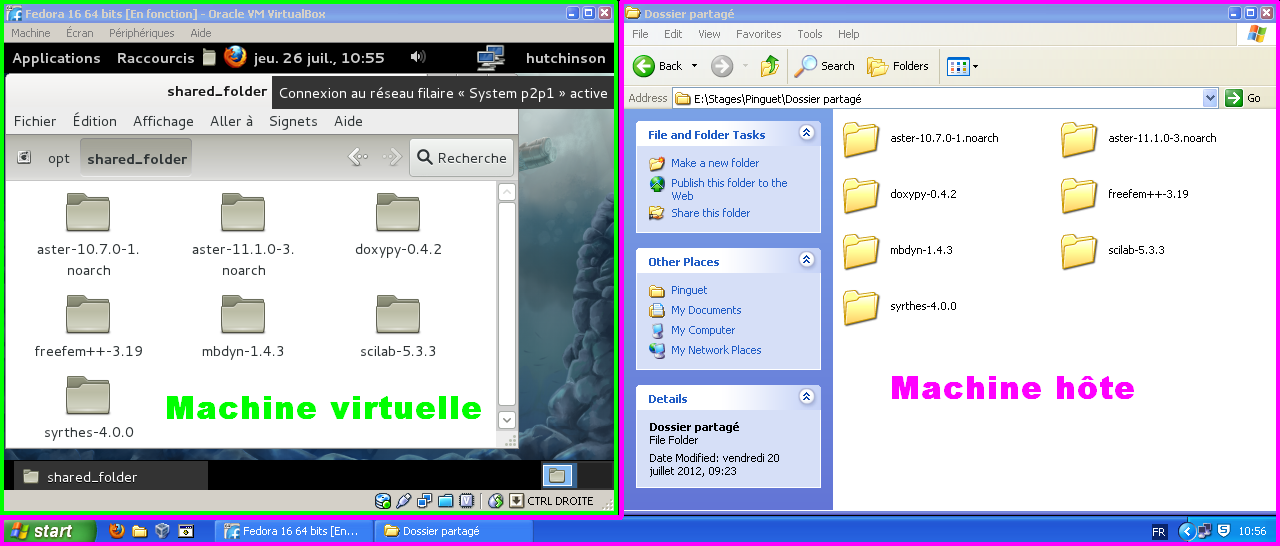
\includegraphics[scale=0.35]{images/Repertoire_partage.png}
	\caption{Répertoire partagé}
	\label{Screenshot Répertoire partagé}
\end{figure}

La capture d'écran de la figure \ref{Screenshot Répertoire partagé} illustre le principe du répertoire partagé.
Dans cet exemple, la machine hôte (Windows) va partager le répertoire \lstinline{E:\Stage\Pinguet\Dossier partage\} avec la machine virtuelle, qui va le monter dans le répertoire \lstinline{/opt/shared\_folder}.
\\


Cela requiert l'installation des \textit{additions invitées} sur la machine virtuelle, aussi appelées \textit{addons}, qui fournissent de nombreux avantages pour les utilisateurs en améliorant la virtualisation :
\begin{itemize}
	\item un affichage graphique de meilleure qualité, dont la 2D et 3D améliorées, l'adaptation de la résolution graphique à celle de la fenêtre ;
	\item le partage du presse-papier ;
	\item la capture ou la libération du pointeur de la souris lorsque l'on entre ou sort de la fenêtre de la machine virtuelle ;
	\item l'utilisation du répertoire partagé.
\\
\end{itemize}





%%%%%%%%%%%%%%%%%%%%%%%%%%%%%%%%%%%%%%%%%%%%%%%%%%%%%%%%%%%%%%%%%%%%%%%%%%%%%%%%%%%%%%%%%%%%%%%%%%%%
%%%%%%%%%%%%%%%%%%%%%%%%%%%%%%%%%%%%%%%%%%%%%%%%%%%%%%%%%%%%%%%%%%%%%%%%%%%%%%%%%%%%%%%%%%%%%%%%%%%%
%%%%%%%%%%%%%%%%%%%%%%%%%%%%%%%%%%%%%%%%%%%%%%%%%%%%%%%%%%%%%%%%%%%%%%%%%%%%%%%%%%%%%%%%%%%%%%%%%%%%
%%%%%%%%%%%%%%%%%%%%%%%%%%%%%%%%%%%%%%%%%%%%%%%%%%%%%%%%%%%%%%%%%%%%%%%%%%%%%%%%%%%%%%%%%%%%%%%%%%%%
%%%%%%%%%%%%%%%%%%%%%%%%%%%%%%%%%%%%%%%%%%%%%%%%%%%%%%%%%%%%%%%%%%%%%%%%%%%%%%%%%%%%%%%%%%%%%%%%%%%%

\section{Étude du problème}

%%%%%%%%%%%%%%%%%%%%%%%%%%%%%%%%%%%%%%%%%%%%%%%%%%%%%%%%%%%%%%%%%%%%%%%%%%%%%%%%%%%%%%%%%%%%%%%%%%%%
%%%%%%%%%%%%%%%%%%%%%%%%%%%%%%%%%%%%%%%%%%%%%%%%%%%%%%%%%%%%%%%%%%%%%%%%%%%%%%%%%%%%%%%%%%%%%%%%%%%%
%%%%%%%%%%%%%%%%%%%%%%%%%%%%%%%%%%%%%%%%%%%%%%%%%%%%%%%%%%%%%%%%%%%%%%%%%%%%%%%%%%%%%%%%%%%%%%%%%%%%

\subsection{Besoin pour les utilisateurs}

Dans l'entreprise Hutchinson, tout particulièrement dans le centre de recherche, des outils scientifiques utilisés ne sont compatibles que sur les systèmes d'exploitation Linux.
C'est le cas par exemple de Code Aster.
Or, le système d'exploitation déployé au sein de l'entreprise est Windows, ce qui ne permet pas d'utiliser ces outils.
\\




%%%%%%%%%%%%%%%%%%%%%%%%%%%%%%%%%%%%%%%%%%%%%%%%%%%%%%%%%%%%%%%%%%%%%%%%%%%%%%%%%%%%%%%%%%%%%%%%%%%%
%%%%%%%%%%%%%%%%%%%%%%%%%%%%%%%%%%%%%%%%%%%%%%%%%%%%%%%%%%%%%%%%%%%%%%%%%%%%%%%%%%%%%%%%%%%%%%%%%%%%
%%%%%%%%%%%%%%%%%%%%%%%%%%%%%%%%%%%%%%%%%%%%%%%%%%%%%%%%%%%%%%%%%%%%%%%%%%%%%%%%%%%%%%%%%%%%%%%%%%%%

\subsection{Première solution}

La première solution qui a été envisagée par la section informatique du centre de recherche, a été de déployer une machine virtuelle, de type VirtualBox ou VMware, sur l'ensemble des ordinateurs.
\\


Cette solution est fonctionnelle, mais possède deux inconvénients non-négligeables :
\begin{itemize}
	\item Tout d'abord, l'ensemble de la machine virtuelle était installée sur un seul et même disque virtuel, ce qui pose un gros problèmes lors du déploiement de la machine virtuelle.
En effet, le système d'exploitation (complet) seul peut atteindre la taille d'une dizaine de GigaOctets, et chacun des outils plusieurs centaines de MégaOctets.
De plus, lors d'une mise à jour d'un simple outil, il est nécessaire de redéployer l'ensemble de la solution, c'est à dire le disque virtuel.
	\item Le second inconvénient repose sur l'utilisation de la machine virtuelle.
Les utilisateurs doivent actuellement configurer et faire fonctionner la machine virtuelle, avant de pouvoir exécuter les outils dont ils ont besoin.
Le programme de virtualisation, comme par exemple VirtualBox, ou même le système d'exploitation Linux utilisé, n'est pas forcément facile à utiliser, et demande tout de même certaines compétences en informatique.
\\
\end{itemize}



%%%%%%%%%%%%%%%%%%%%%%%%%%%%%%%%%%%%%%%%%%%%%%%%%%%%%%%%%%%%%%%%%%%%%%%%%%%%%%%%%%%%%%%%%%%%%%%%%%%%
%%%%%%%%%%%%%%%%%%%%%%%%%%%%%%%%%%%%%%%%%%%%%%%%%%%%%%%%%%%%%%%%%%%%%%%%%%%%%%%%%%%%%%%%%%%%%%%%%%%%
%%%%%%%%%%%%%%%%%%%%%%%%%%%%%%%%%%%%%%%%%%%%%%%%%%%%%%%%%%%%%%%%%%%%%%%%%%%%%%%%%%%%%%%%%%%%%%%%%%%%

\subsection{Solution envisagée}
\label{Solution envisagée}

En analysant la solution actuelle, tout particulièrement les deux problèmes principaux, notre objectif était donc de trouver un moyen de contourner ces problèmes, pour en faire des avantages.
\\


Premièrement, comme expliqué dans la partie \ref{Particularités de la virtualisation}, il est possible d'utiliser les disques virtuels comme de vrais disques-dur, que l'on peut monter dans la machine virtuelle, pour que le disque apparaisse dans l'arborescence des fichiers de Linux, de la même façon qu'une clé USB apparait dans le "Poste de travail" sur Windows.

De ce principe, il serait intéressant d'installer le système d'exploitation sur un disque virtuel, puis l'ensemble des outils utilisés sur des disques virtuels distincts.

Ainsi, le déploiement de l'ensemble de la solution ne s'effectuera qu'une seule fois, puis à chaque mise à jour ou ajout d'un outil, seul son disque dur virtuel (de "petite" taille) sera déployé.
\\


Aux difficultés d'utilisation de la machine virtuelle, viennent s'ajouter les actions de montage et démontage des disques virtuels.

Pour obtenir une solution simple d'utilisation, il est possible d'automatiser les phases de paramétrisation et de contrôle de la machine virtuelle.
De plus, une fois la solution fonctionnelle, une interface graphique permettrait à l'utilisateur d'effectuer les actions de manière simple et automatique.
\\


\begin{figure}[!h]
	\center
	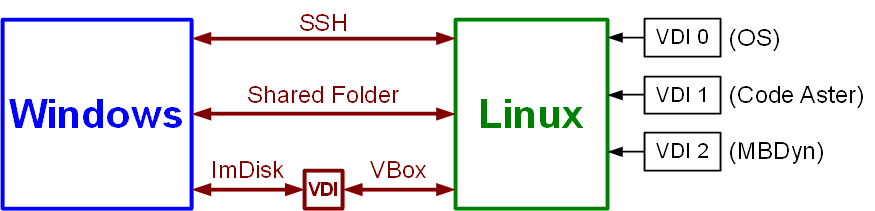
\includegraphics[scale=0.5]{images/Solution_envisagee.png}
	\caption{Schéma de la solution envisagée}
	\label{Schéma Solution envisagée}
\end{figure}

La figure \ref{Schéma Solution envisagée} illustre le principe de la solution envisagée, où le système d'exploitation de la machine hôte Windows pourra échanger des fichiers avec la machine virtuelle Linux, sur laquelle on pourra y brancher différents disques virtuels et exécuter les calculs.